\paragraph{Model}

\begin{align}
\bF_t &= \sum_{i=1}^{N_c}\balpha_i (C_{i,t} + \beta_i) +  \ve{\varepsilon}_t, \qquad &\ve{\varepsilon}_t \sim \mathcal{N}(\ve{0},\sig^2 \bI)   \\
C_{i,t} &= \gam_i C_{i,t-1} + n_{i,t}, & n_{i,t} \sim \text{Poisson}(n_{i,t}; \lam_i \Del)
\end{align}

implicit assumption that $\bn_i \perp \bn_j, \, \forall i\neq j$

\paragraph{Inference}

let $\bn=(n_{1,1}, n_{2,1}, \ldots, n_{N_c,1}, n_{1,2}, \ldots, n_{N_c,T})\T$. 
similar def of $\bC$.

\begin{align} \label{eq:M2}
\ve{M} = %- \bb=
\begin{bmatrix}
1 & 1 & 0 & 0 & \cdots & \cdots \\
1 & -\gamma_1 & 1 & -\gam_2 & \ldots & 1 & -\gam_{N_c}  & 0 & \cdots \\
\vdots & \vdots & \vdots & \vdots & \vdots  \\
0 & 0 & 0 \ldots & 1 & -\gamma_{N_c-1} & 1 & -\gamma_{N_c}
\end{bmatrix}
\end{align} 

inference as before, but replacing the scalar $\beta$ with $\bbeta=(\beta_1, \ldots, \beta_{N_c})\T$, and making minor adjustments to deal with dimensionality issues.

\paragraph{Learning}

estimating $\balpha=(\balpha_1,\ldots,\balpha_{N_c})\T$ is similar.  now, we compute $\hbalpha_x=(\halpha_{1,x}, \ldots, \halpha_{N_c,x})\T$ using

\begin{align}
\hbalpha_x = (\bC + \widetilde{\bbeta})\backslash \bF_x,
\end{align}

\noindent where $\widetilde{\bbeta}$ is $\bbeta$ reparameterized to be the same size as $\bC$.

estimating $\bbeta$ proceeds as before, but since it is a vector, we use Matlab's \texttt{quadprog}, imposing the constraint that $\beta_i>0 \, \forall i$.

\begin{figure}[H]
\centering 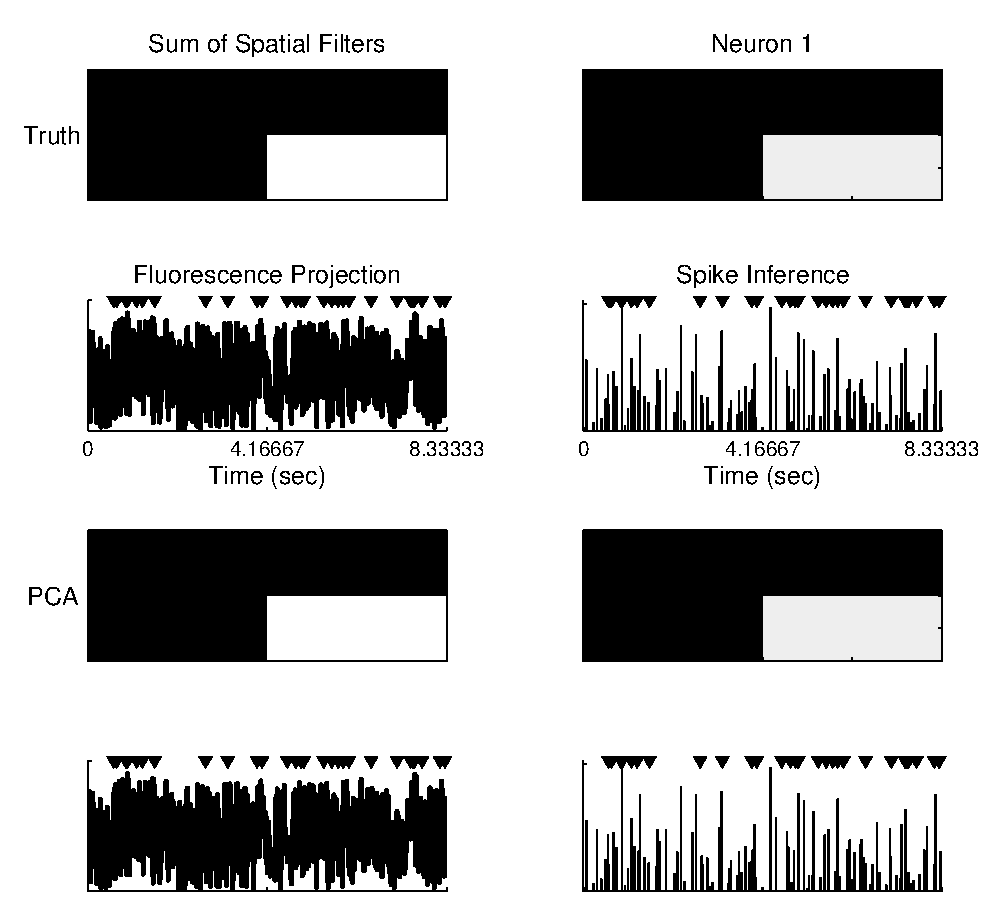
\includegraphics[width=.9\linewidth]{../figs/spatial_multi}
\caption{Simulation showing that even when two neuron's spatial filters are largely overlapping} \label{fig:spatial_multi}
\end{figure}

%\begin{figure}[H]
%\centering 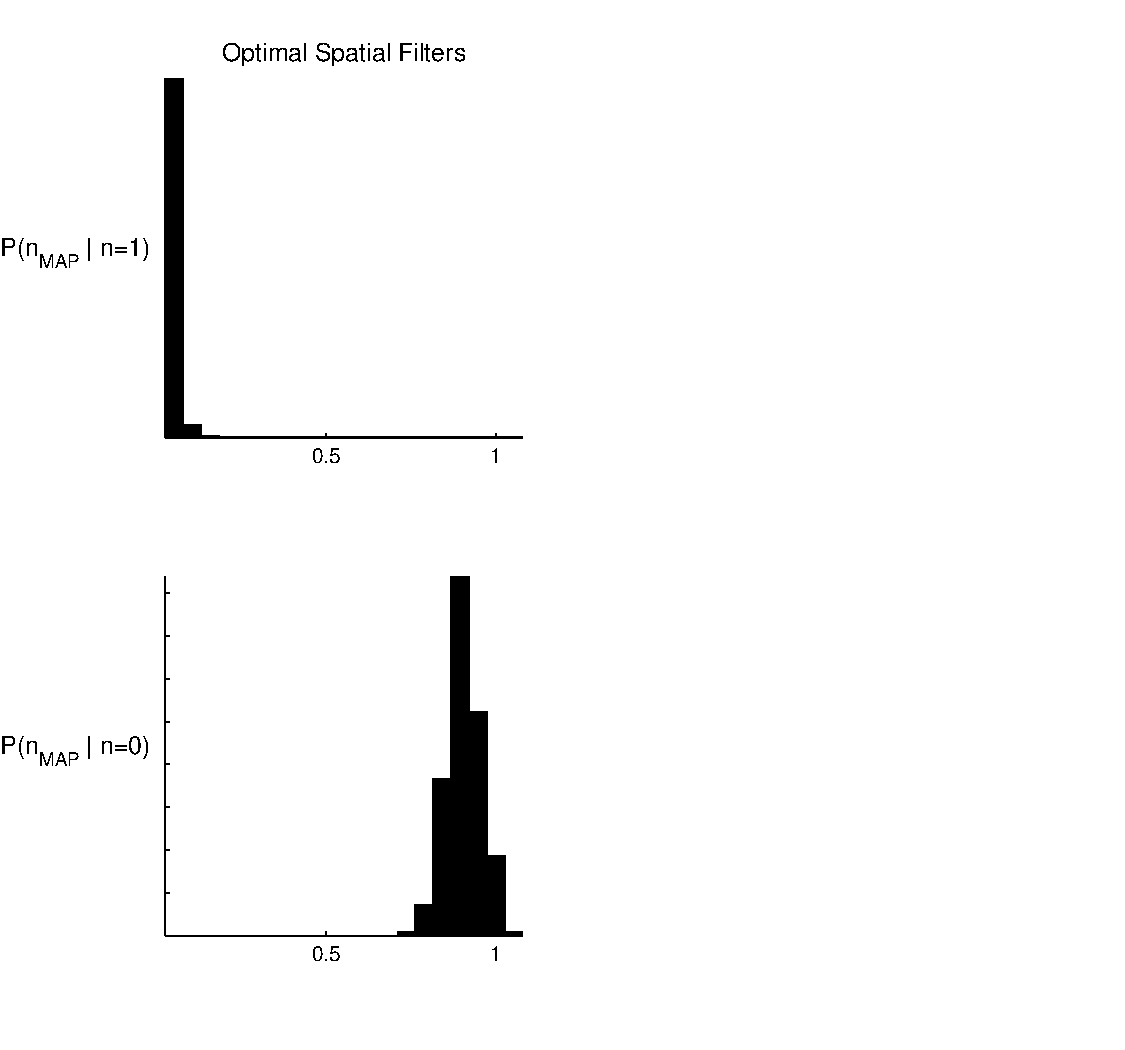
\includegraphics[width=.9\linewidth]{../figs/multi_hist1}
%\caption{same as spatial EM, but with 2 cells in ROI} \label{fig:spatial_multi}
%\end{figure}

